\chapter{综合题}

\begin{Ex}
  给出以下四个图的顶点最小度、顶点连通度、边连通度、色数,并说明它们是否为连通图、
  偶图、欧拉图、哈
  密顿图、可平面图。
  
\vspace{0.5cm}
    \begin{minipage}{0.49\linewidth}
    \centering
    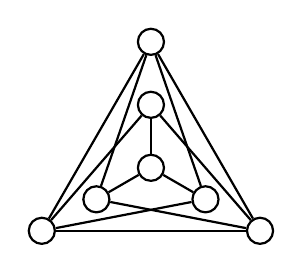
\begin{tikzpicture}[auto,
    specification/.style ={circle, draw, thick}, scale = 0.8]
   \node[specification] (A)  at (0,0)  {};
   \node[specification] (B)  at (90:2cm)  {};
   \node[specification] (C)  at (210:2cm)  {};
   \node[specification] (D)  at (330:2cm)  {};
   \node[specification] (E)  at (90:1cm)  {};
   \node[specification] (F)  at (210:1cm)  {};
   \node[specification] (G)  at (330:1cm)  {};


   \draw[thick] (B) to  (C);
   \draw[thick] (C) to  (D);
   \draw[thick] (D) to  (B);
   
   
   \draw[thick] (E) to (C);
   \draw[thick] (E) to (D);

   \draw[thick] (A) to (E);
   \draw[thick] (A) to (F);
   \draw[thick] (A) to (G);

   \draw[thick] (B) to (F);
   \draw[thick] (B) to (G);

   \draw[thick] (C) to (G);
   \draw[thick] (D) to (F);

      


   
 \end{tikzpicture}

 (a)
\end{minipage}\hfill
    \begin{minipage}{0.49\linewidth}
    \centering
    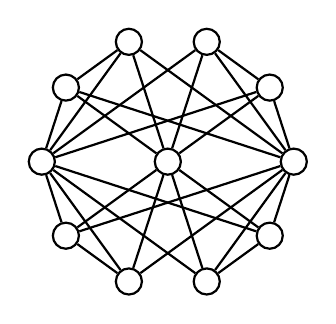
\begin{tikzpicture}[auto,
    specification/.style ={circle, draw, thick}, scale = 0.8]
   \node[specification] (A)  at (0:2cm)  {};
   \node[specification] (B)  at (36:2cm)  {};
   \node[specification] (C)  at (2*36:2cm)  {};
   \node[specification] (D)  at (3*36:2cm)  {};
   \node[specification] (E)  at (4*36:2cm)  {};
   \node[specification] (F)  at (5*36:2cm)  {};
   \node[specification] (G)  at (6*36:2cm)  {};
   \node[specification] (H)  at (7*36:2cm)  {};
   \node[specification] (I)  at (8*36:2cm)  {};
   \node[specification] (J)  at (9*36:2cm)  {};
   \node[specification] (O)  at (0,0)  {};

   \draw[thick] (O) to  (B);
   \draw[thick] (O) to  (C);
   \draw[thick] (O) to  (D);
   \draw[thick] (O) to  (E);
   \draw[thick] (O) to  (G);
   \draw[thick] (O) to  (H);
   \draw[thick] (O) to  (I);
   \draw[thick] (O) to  (J);

   \draw[thick] (A) to  (B);
   \draw[thick] (B) to  (C);
   \draw[thick] (A) to  (J);
   \draw[thick] (J) to  (I);

   \draw[thick] (D) to  (E);
   \draw[thick] (E) to  (F);
   \draw[thick] (F) to  (G);
   \draw[thick] (G) to  (H);

   \draw[thick] (A) to  (C);
   \draw[thick] (A) to  (D);
   \draw[thick] (A) to  (E);
   \draw[thick] (A) to  (G);
   \draw[thick] (A) to  (H);
   \draw[thick] (A) to  (I);


   \draw[thick] (F) to  (B);
   \draw[thick] (F) to  (C);
   \draw[thick] (F) to  (D);
   \draw[thick] (F) to  (H);
   \draw[thick] (F) to  (I);
   \draw[thick] (F) to  (J);
 \end{tikzpicture}

 (b)
\end{minipage}


    \begin{minipage}{0.49\linewidth}
    \centering
    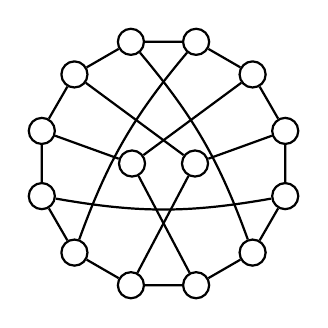
\begin{tikzpicture}[auto,
      specification/.style ={circle, draw, thick}, scale=0.8]

   \node[specification] (A)  at (15:2cm)  {};
   \node[specification] (B)  at (15+30:2cm)  {};
   \node[specification] (C)  at (15+2*30:2cm)  {};
   \node[specification] (D)  at (15+3*30:2cm)  {};
   \node[specification] (E)  at (15+4*30:2cm)  {};
   \node[specification] (F)  at (15+5*30:2cm)  {};
   \node[specification] (G)  at (15+6*30:2cm)  {};
   \node[specification] (H)  at (15+7*30:2cm)  {};
   \node[specification] (I)  at (15+8*30:2cm)  {};
   \node[specification] (J)  at (15+9*30:2cm)  {};
   \node[specification] (K)  at (15+10*30:2cm)  {};
   \node[specification] (L)  at (15+11*30:2cm)  {};
   \node[specification] (X)  at (-0.5cm, 0cm)  {};
   \node[specification] (Y)  at (0.5cm, 0cm)  {};
   
   


   \draw[thick] (A) to  (B);
   \draw[thick] (B) to  (C);
   \draw[thick] (C) to  (D);
   \draw[thick] (D) to  (E);
   \draw[thick] (E) to  (F);
   \draw[thick] (F) to  (G);
   \draw[thick] (G) to (H);
   \draw[thick] (H) to (I);
   \draw[thick] (I) to  (J);
   \draw[thick] (J) to  (K);
   \draw[thick] (K) to  (L);
   \draw[thick] (L) to  (A);

   \draw[thick] (C) to [bend right = 10] (H);
   \draw[thick] (D) to [bend left = 10] (K);
   \draw[thick] (G) to [bend right = 10] (L);

   \draw[thick] (X) to  (B);
   \draw[thick] (X) to  (F);
   \draw[thick] (X) to  (J);

   \draw[thick] (Y) to  (A);
   \draw[thick] (Y) to  (E);
   \draw[thick] (Y) to  (I);
 \end{tikzpicture}

 (c)
\end{minipage}\hfill
    \begin{minipage}{0.49\linewidth}
      \centering
          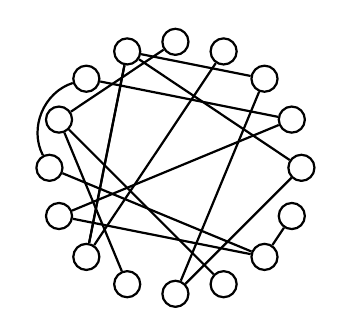
\begin{tikzpicture}[auto,
      specification/.style ={circle, draw, thick}, scale=0.8]

   \node[specification] (A)  at (0:2cm)  {};
   \node[specification] (B)  at (360/16:2cm)  {};
   \node[specification] (C)  at (360/16*2:2cm)  {};
   \node[specification] (D)  at (360/16*3:2cm)  {};
   \node[specification] (E)  at (360/16*4:2cm)  {};
   \node[specification] (F)  at (360/16*5:2cm)  {};
   \node[specification] (G)  at (360/16*6:2cm)  {};
   \node[specification] (H)  at (360/16*7:2cm)  {};
   \node[specification] (I)  at (360/16*8:2cm)  {};
   \node[specification] (J)  at (360/16*9:2cm)  {};
   \node[specification] (K)  at (360/16*10:2cm)  {};
   \node[specification] (L)  at (360/16*11:2cm)  {};
   \node[specification] (M)  at (360/16*12:2cm)  {};
   \node[specification] (N)  at (360/16*13:2cm)  {};
   \node[specification] (O)  at (360/16*14:2cm)  {};
   \node[specification] (P)  at (360/16*15:2cm)  {};
   
   


   \draw[thick] (A) to  (F);
   \draw[thick] (C) to  (F);
   \draw[thick] (F) to  (K);
   \draw[thick] (C) to  (M);
   \draw[thick] (A) to  (M);
   \draw[thick] (D) to  (K);
   \draw[thick] (F) to  (K);


   
   \draw[thick] (H) to  (E);
   \draw[thick] (H) to (L);
   \draw[thick] (H) to (N);
   
   \draw[thick] (P) to  (O);
   \draw[thick] (B) to  (G);
   \draw[thick] (G) to [bend right = 50] (I);
   \draw[thick] (I) to  (O);
   \draw[thick] (O) to  (J);
   \draw[thick] (J) to  (B);

 \end{tikzpicture}
 (d)
\end{minipage}

\end{Ex}

\begin{Ex}
  珍珠四颗,有真有假,不能用眼鉴别。真珍珠重量相同且为p,假珍珠重量也相同且为q,
  $p > q$。用秤(不是天平)仅称三次,称出真假,应该怎样做?
\end{Ex}


%%% Local Variables:
%%% mode: latex
%%% TeX-master: "book"
%%% End:
